\section{Results}
\label{sec:results}

\subsection{Comparison identity alone does not license an atomistic proof}
\label{sec:primary}

The primary controlled comparison asks whether a measurement from the correct structure pair is necessarily suitable evidence. It is not. For Qwen, the comparison-ID checker accepted 393 numerical answers, but 81 were invalid under the supplied proof rules. The full-definition checker accepted 312: all 312 had correct verdicts and licensed proofs (Fig.~\ref{fig:checks}). Of the 81 additionally rejected acceptances, 42 had incorrect verdicts; the other 39 had verdicts that happened to be correct but relied on an incompatible measurement or operation. The latter errors would be invisible if evaluation checked only the final label.

All three checkers acted on identical raw evidence selections. The additional exclusions therefore arise from requiring the selected atom set, reference frame, alignment, periodic handling, weighting, and mathematical relation to match the claim, not from a new language-model prediction or an additional evidence search. The 81 prevented invalid acceptances equal 4.60 percentage points of all 1,760 cases (95\% source-group bootstrap interval 3.58--5.57). Full checking lost none of the 312 licensed answers. Within this defined task, run identity is necessary for using a record about the requested comparison, but is insufficient to establish that the selected quantity proves the claim.

\begin{figure}[tbp]
  \centering
  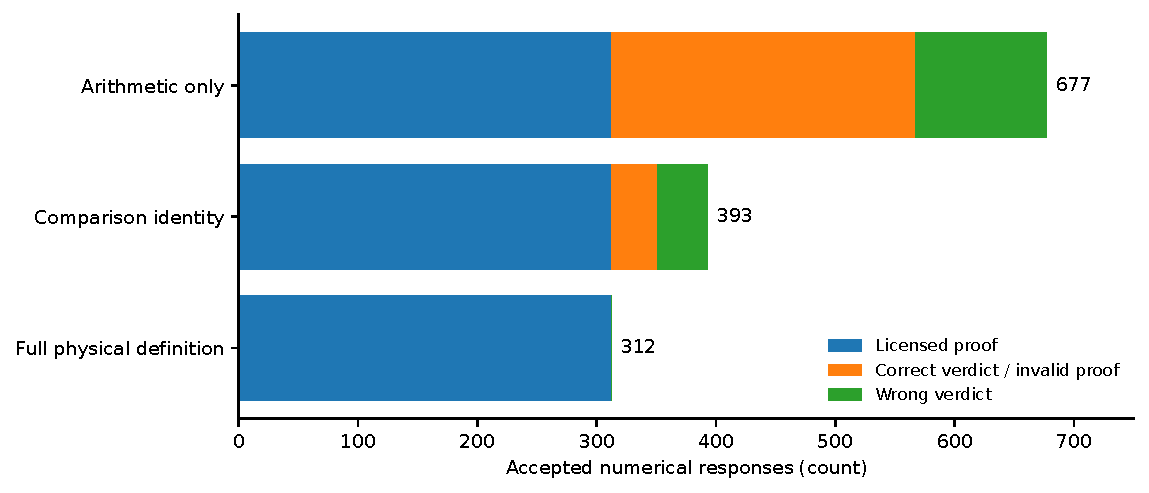
\includegraphics[width=\linewidth]{figure_02.pdf}
  \caption{Qwen numerical acceptances under arithmetic-only, comparison-ID, and full-definition checks on identical evidence selections. Stacked segments distinguish correctly licensed answers, wrong verdicts, and correct verdicts with unlicensed proofs.}
  \label{fig:checks}
\end{figure}

\subsection{Validation filters bad answers but does not recover missing proofs}
\label{sec:coverage_results}

The safety gain comes with a coverage cost. Of the 81 Qwen acceptances excluded only by full checking, 60 concerned answerable cases and 21 concerned insufficient-evidence cases. Thus, among the 1,100 answerable cases, accepted numerical answers decreased from 372 (33.82\%) under comparison-ID checking to 312 (28.36\%) under full checking, a decrease of 5.45 percentage points (95\% interval 4.09--6.91). The 312 retained answers are the same licensed answers in both conditions; the stricter checker supplies no replacement proof for the 60 newly rejected answerable cases.

The low coverage is not unique to Qwen. Full-definition valid numerical coverage was 121/1,100 (11.00\%) for Phi and 168/1,100 (15.27\%) for SmolLM (Supplementary Fig.~S2), against 312/1,100 for Qwen (95\% interval 25.73--31.00\%). Relative to comparison-ID checking, full checking prevented 245 additional invalid acceptances for Phi and 273 for SmolLM, again without rejecting any licensed answers. These are selective-filter results: correctness is assessed \emph{among accepted numerical answers}, not as 100\% overall task accuracy.

A deterministic oracle that enumerates permitted public-record proofs resolved all 1,760 cases, including all 1,100 answerable and all 660 insufficient-evidence cases. A valid proof therefore existed in the supplied packet for every answerable case, although the evaluated model--checker pipelines often failed to identify it. The oracle is a strong programmatic baseline for this constructed task and is not a trained language model.



\subsection{The physical definition changes what RMSD measures}
\label{sec:physical_results}

The coordinate evidence exhibits the underlying distinction. Across 55 source groups, stored-frame adsorbate RMSD exceeded aligned internal RMSD by more than a factor of ten in 16 groups; the median ratio was 3.27 (Supplementary Fig.~S1). Stored-frame RMSD retains positional and orientational displacement. In contrast, internal RMSD uses an unwrapped adsorbate followed by a proper rigid alignment, which removes overall translation and rotation.\cite{kabsch1978discussion} Equal distance units therefore do not make the quantities interchangeable.

The original system-by-system coordinates were not available in the frozen inputs used to regenerate figures; Supplementary Fig.~S1 accordingly displays only the documented aggregate statistics. This empirical comparison illustrates the motivation for testing physical definitions, but does not itself establish a universal inequality between stored-frame and internal RMSD. The shared-frame adsorbate and mobile-atom RMSDs, by contrast, admit explicit subset bounds because the adsorbate's equal-weight squared displacements are included in the mobile-atom sum (Eq.~\ref{eq:bounds}). The geometries are UMA-relaxed coordinates, not independent density-functional-theory validation of structural accuracy or adsorption energetics.



\subsection{Directly correct verdicts frequently lack valid proofs}
\label{sec:direct_results}

Direct-answer evaluation produces a second gap between an answer and its justification. Three-way verdict accuracy was 38.81\% for Qwen, 32.56\% for Phi, and 20.45\% for SmolLM. Requiring a valid proof on decisive claims, or a correct insufficiency response when appropriate, reduced proof-aware accuracy to 17.39\%, 23.01\%, and 3.75\%, respectively (Fig.~\ref{fig:direct}). The scores use all 1,760 variants, and proof-aware accuracy must not be confused with valid \emph{numerical} coverage of the 1,100 answerable cases.

Qwen gave numerical answers on 1,096 answerable cases, but only 255 combined a correct verdict with a licensed proof. It also gave numerical answers for 607 of 660 insufficient-evidence cases. Phi had 405 proof-aware successes in total, including 26 valid numerical answers and 379 correct insufficiency responses. These examples show how overall verdict scores can conceal the different outcomes of guessing a correct label, producing a valid proof, and correctly recognizing that the evidence cannot decide a claim.

The direct-answer and evidence-selection prompts were independent model requests. Therefore differences between direct performance and check-assisted selection performance cannot be interpreted as a causal effect of adding a checker. The matched causal isolation applies specifically to the three deterministic checkers processing the same selected records.

\begin{figure}[tbp]
  \centering
  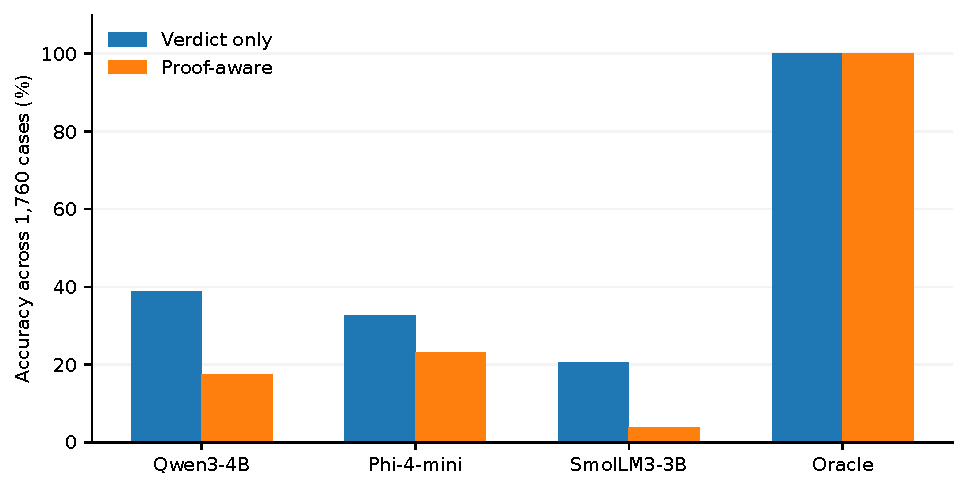
\includegraphics[width=\linewidth]{figure_03.pdf}
  \caption{Direct three-way verdict accuracy and proof-aware accuracy over 1,760 variants, compared with the deterministic oracle. Error bars indicate 95\% source-group bootstrap intervals.}
  \label{fig:direct}
\end{figure}

\subsection{Evidence presentation changes valid-answer coverage}
\label{sec:presentation_results}

The same underlying numerical facts did not yield equal success across presentations. Qwen's valid numerical coverage was 33.09\% on structured evidence versus 23.64\% on report-form evidence, a paired difference of 9.45 percentage points (95\% interval 4.73--13.82; Supplementary Fig.~S3). SmolLM showed a difference of 8.36 points (4.91--12.00). Phi's difference was $-0.18$ points ($-4.73$ to 3.82). Both presentations retained the relevant physical facts; however, the report rendering also omitted redundant metric names. Accordingly, the observed differences cannot be attributed to prose formatting alone.

The comparison is exploratory. It identifies a presentation-associated difference in selection success under the frozen prompts, but does not isolate the role of verbosity, naming cues, or an intrinsic change in physical reasoning.



\subsection{Selection failures depend on the permitted operation}
\label{sec:family_results}

Task-family performance was uneven (Supplementary Fig.~S4). Phi produced no licensed adsorbate upper-bound answer (0/220), while SmolLM produced no licensed mobile lower-bound answer (0/220). Qwen produced licensed answers in all four answerable families, with coverage ranging from 26.36\% for unit conversion to 34.55\% for mobile lower bounds. The oracle solved every family under the stated operation rules.

These outcomes identify which combinations of supplied records and permitted operations were difficult under this protocol. Bounds demand more than correct multiplication or comparison: the source and target atom sets, direction of the bound, and measurement convention must also match. These error patterns do not reveal the models' private reasoning or establish performance on general scientific problems.


